\documentclass[xcolor=dvipsnames]{beamer}
\usetheme{Berlin}  %% Themenwahl
%\definecolor{htwgreen}{rgb}{118,185,0}
\definecolor{htwgreen}{rgb}{0.461,0.723,0}
\usecolortheme[named=htwgreen]{structure}

\setbeamertemplate{navigation symbols}{}%remove navigation symbols
%show frame numbers
\expandafter\def\expandafter\insertshorttitle\expandafter{%
\insertshorttitle\hfill%
\insertframenumber\,/\,\inserttotalframenumber}

\usepackage[utf8]{inputenc}
\usepackage[ngerman]{babel} %german language
\usepackage{graphicx} %insert pictures
%\usepackage{svg} %insert vector graphics
\usepackage[export]{adjustbox} %for columns?
\usepackage{listings} %insert code
\lstset{keepspaces=true, numbers=left} %configure code listings

\title{Parallelisierung der Schwingung einer Gitarrensaite}
\author{Patrick Fehling \& Christian Schütt}
\date{\today}

\begin{document}
\maketitle
\frame{\tableofcontents}

\section{Grundlagen}
\begin{frame}\frametitle{Aufgabe}
		\textbf{Aufgabe:}\\
		Visualisierung der Amplituden einer vibrierenden Saite auf Grundlage der Wellengleichung im eindimensionalen Fall\\
		\vspace{1ex}
		$A(i, t + 1) = 2A(i, t) - A(i, t - 1) + c(A(i - 1, t) - 2A(i, t) + A(i + 1, t))$\\
		\vspace{2ex}
		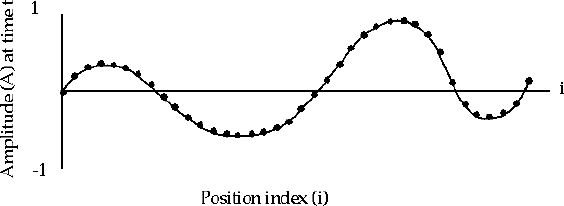
\includegraphics[width=1.0\textwidth,valign=t]{pictures/wellengleichung_aufgabe}
\end{frame}

\begin{frame}\frametitle{Rahmenbedingungen}
	\begin{itemize}
		\item sequentielle Implementierung
		\item parallelisierte Implementierungen (OpenMP und...)
		\item Graphical User Interface
		\item Konfiguration per Benutzeroberfläche oder Konfigurationsdatei
		\item optional: Perturbationen
		\vspace{3ex}
		\item Performancevergleich
		\item Präsentation, Paper, Dokumentation
	\end{itemize}
\end{frame}

\section{Implementierung}
\begin{frame}\frametitle{Implementierung}
	\begin{itemize}
		\item
		%Herangehenweise
		%Datenstrukturen
		%Parallelisierung
		%Snippets
	\end{itemize}
\end{frame}

\section{Vergleich}
\begin{frame}\frametitle{Vergleich}
	%Diagramm 1
\end{frame}

\begin{frame}\frametitle{Vergleich}
	%Diagramm 2
\end{frame}

\section{Demo}
\section{Fazit \& Ausblick}

\begin{frame}
	\frametitle{Einführung}
	\begin{Definition}
		Definition..
	\end{Definition}
	Hier kommt eine Lücke:
	\vspace{4ex}
	\begin{itemize}
		\item Listenelement 1
		\item Listenelement 2
	\end{itemize}
\end{frame}

\frame{\tableofcontents[current]}

\begin{frame}\frametitle{Columns}
	\begin{columns}[t,onlytextwidth]
		\column{.5\textwidth}
			Text auf linker Seite\\
			Da ist ein Bild $\rightarrow$
		\column{.5\textwidth}
		\centering
		
\includegraphics[width=1.0\textwidth,valign=t]{pictures/placeholder}
	\end{columns}
\end{frame}

\begin{frame}[fragile]\frametitle{Codelisting}
\begin{lstlisting}[language=Java]
public int method(int arg0){
    Object object = new Object();
    return object.anotherMethod(arg0);
}
\end{lstlisting}
\end{frame}

\begin{frame}\frametitle{Zusammenfassung}
	\begin{itemize}
		\item Punkt 1
	\end{itemize}
\end{frame}

\begin{frame}
	\centering
	\textcolor{htwgreen}{{\LARGE Vielen Dank für Ihre Aufmerksamkeit!\\[6ex] Fragen?}}
\end{frame}

\begin{frame}\frametitle{Quellen}
		\begin{itemize}
		\item Quelle 1
	\end{itemize}
\end{frame}

\end{document}